\documentclass[a4paper, 12pt]{article}
\usepackage{graphicx} 

\usepackage[english, russian]{babel}
\usepackage[T2A]{fontenc}
\usepackage[utf8]{inputenc}
\usepackage{indentfirst}
\usepackage{ragged2e}

% \usepackage[english, russian]{babel}
% \usepackage{fontspec}
% \setmainfont{Times New Roman}

\usepackage{amsmath, amsfonts, amssymb, amsthm, mathtools}

\usepackage[
    sorting=none
]{biblatex}
\addbibresource{References.bib}

\usepackage{geometry}
\geometry{top=20mm}
\geometry{bottom=20mm}
\geometry{left=30mm}
\geometry{right=10mm}

\usepackage{ulem}

\linespread{1.5}
\setlength{\parindent}{20pt}
\hyphenation{}

% \usepackage{titleps}
% \newpagestyle{main} {
%     \setheadrule{0.4pt}
%     \sethead{}{}{}
%     \setfootrule{0.4pt}
%     % \setfoot{}{center}{}
% }
% \pagestyle{main}

\pagenumbering{arabic}


\begin{document}
\thispagestyle{empty}

\begin{center}

\textbf{ПРАВИТЕЛЬСТВО РОССИЙСКОЙ ФЕДЕРАЦИИ}

\vspace{1\baselineskip}
\textbf{Федеральное государственное автономное образовательное
учреждение высшего образования}

\vspace{1\baselineskip}
\textbf{Национальный исследовательский университет \\
«Высшая школа экономики»}

\vspace{1\baselineskip}
\textbf{Факультет компьютерных наук \\
Образовательная программа \\
«Прикладная математика и информатика»}

\vspace{1\baselineskip}
\textbf{КУРСОВАЯ РАБОТА} \\

\vspace{1\baselineskip}
На тему: \uline{Различные способы построения графовых структур данных для поиска ближайшего соседа} \\
Тема на английском: \uline{Several Ways to Form Graph Based Nearest Neighbour Search Structure} 
\end{center}



\vspace{7\baselineskip}

\begin{flushright}
    \uline{Студент} / студентка \uline{2-го} курса \\
    группы № \underline{БПМИ2110/21ПМИ-2}: \\
    $\underset{\text{(Ф.И.О.)}}{\uline{\text{Рябков Игорь Дмитриевич}}}$
    
    Научный руководитель: \\
    $\underset{\text{(Ф.И.О.)}}{\uline{\text{Пономаренко Александр Александрович}}}$ \\ 
    $\underset{\text{(должность, звание)}}{\uline{\text{Доцент, НН Кафедра прикладной математики и информатики}}}$ \\ 
\end{flushright}

\newpage

\tableofcontents

\newpage

\newpage
\section{Введение}



\newpage
\section{Основная часть}

\subsection{История развития структур для поиска ближайшего соседа}


\subsection{Феномен тесного мира}

Для того, чтобы понять, каким должен быть граф для 
оптимальной работы нашего алгоритма, я предлагаю обратиться
к структурам, которые возникают само собой в приро\-де, 
к графам, которые формирет общество.

\subsubsection{Теория 6 рукопожатий}

Венгерский писатель Karinthy Frigyes Ernő в 1928г в рассказе 
"Звенья цепи" впервые сформулировал данную проблему. Согласно ей, 
любые два человека на планете связаны через 5-6 общих знакомых.

Рассуждая над этой проблемой, Stanley Milgram - американский 
социальный психолог и педагог в своей статье "The Small World Problem" \cite{Milgram}
описал проведённый им эксперимент: 
Он выдал 300 писем жителям из разных городов и попросил доставить 
их одному человеку из Бостона (США). Важным условиям было то, что
люди могли передавать письма только своим знакомым, которые по их
мнению могли знать целовека-цель.
По результатам исследование, даже не смотря на то, что до места назначения
дошли далеко не все письма, те, которым это удалось, прошли в среднем через цепь из
5-6 человек. 

Данные наблюдения кажутся очень полезными для нас. Ведь если нам
удастся воссоздать граф, который с хорошей точностью моделируют
общественные сети, мы сможем из любой вершины графа добираться до 
цели за сравнимо малое число посредников. Причём для этого нам даже 
не придётся использовать сложные алгоритмы поиска. Вспомним эксперимент
Милгрема, в нём каждый человек не пытался искать оптимальный путь
от него до цели, он лишь отправлял письма тем знакомым, которые казались
ближе к месту назначения. Формально - это простой жадный поиск, который
в эксперименте Милгрема прошёлся всего лишь по 5-6 промежуточным значениям
и, что не мало важно, достиг цели.

% Однако, при попытке смоделировать данное поведение на компьютере, даже
% на небольшой выборке значений, это не сработает. Если мы построим
% граф, который будет состоять из кластеров вершин (вершины, соеденины
% ребром только в случае, если они находятся рядом), его диаметр будет
% всё равно очень большим. То есть, чтобы добраться от одной вершины
% к другой, понадобиться много посредников

\subsubsection{Случайные графы Erdős–Rényi}
Попробуем предположить, что общественные сети можно
представить, как случайный граф $G(n, p) = \{V, E\}$ состоящий из $n$ вершин, с
вероятностью проведения ребра p. Логично предположить, что $np = const = \lambda$.
Можно объяснить это так: структура графа не должна зависить от кол-ва
вершин в нём. Он всегда должен выглядеть примерно одинаково ($deg(v) \approx const$). Ну или ещё
одно описание: кол-во моих друзей не увеличится, если население планеты 
увеличится в несколько раз. Обоснуем это формально:
\begin{equation}
    P(deg(v) = k) = \binom{n}{k}p^k(1-p)^{1-k}
    \Rightarrow deg(v) \sim Bin(p)
\end{equation}
Так как $np = const = \lambda : \mathbb{E}[deg(v)] = np = \lambda$

Так мы описали граф, изучением которого занимались
два великих Венгерских математика Paul Erdős и Alfréd Rényi. (Причём $\lambda$ обычно
выбирается много меньше чем $n$, ведь наш круг общения никчёмно мал по сравнению с 8 млрд. людей
планете) 

Разультаты, к которым пршли данные математики показали, что случайные графы имеют 
сравнительно малый средний диаметр графа $d(G)$. Где
\begin{equation}
    d(G) = \frac{1}{|V|}\sum_{u, v \in V}d(u, v)
\end{equation}
\begin{equation}
    d(u, v) = \min_{k \in \mathbb{R}}\{\exists a_i, \ i = \overline{1k}  : a_1 = u, a_{k + 1} = v, (a_i, a_{i + 1}) \in E\}
\end{equation}
Казалось бы, малый диаметр - всё, что нам нужно. И это было бы так, если бы мы не 
использовали жадный алгоритм для поиска. Случайные рёбра в графе помогают 
нам легко и быстро приблизиться к месту назначения, однако отсутствие локальных
рёбер приводит к большому кол-ву локальных минимумов, что ведёт за собой большую
погрешность полученном результате, пример:

\begin{figure}[H]
\centering
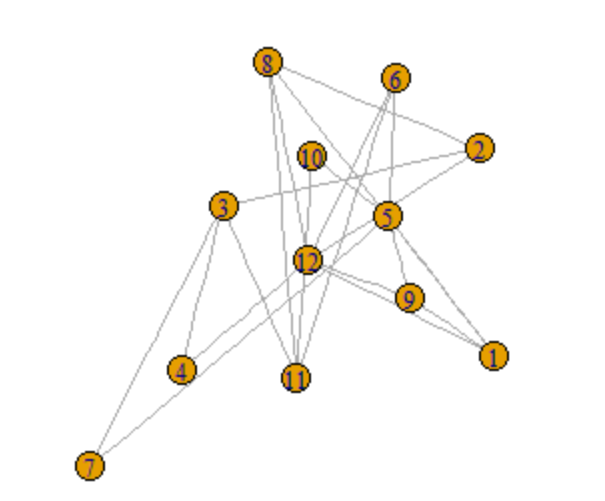
\includegraphics[scale=0.3]{./pictures/random_graph.png}
\caption{Случайный граф} \label{random_graph}
\end{figure}

Взглянув на рисунок \ref{random_graph}, можно заметить, что если мы хотим добраться до вершины 3,
используя жадный поиск, то это нам удастся только из непосредственных соседей вершины номер 3.
Это говорит о том, что такой граф хорош в навигации на больших масштабах, но плох при локальном
поиске. Что не состыкуется с теорией 6 рукопожатий

Ошибка в наших рассуждениях была в том, что мы предположили, что связи между людьми абсолютно
случайны, но ведь это не так. Милгрэм, описывая результаты своего эксперимента, делал акцент
на то, что общественные графы состоят из кластеров. Это можно описать так: Вероятность знакомства
с человеком тем больше, чем мы ближе; А также, вероятность, того, что люди дружат прямо пропорциональна
кол-ву их общих друзей. Наличие данной концепции образовало бы больше локальных рёбер, что решило бы
проблему локальных минимумов. Формально это можно описать, через коэффицент кластеризации вершины:
\begin{equation*}
    cc(v) = \frac{\#\{(x, y) \in E, \ x, y \in V: (x, v), (y, v) \in E\}}
    {\#\{(x, y), \ x, y \in V: (x, v), (y, v) \in E\}}
\end{equation*}
По аналогии коэффицент кластеризации графа:
\begin{equation*}
    cc(G) = \frac{1}{|V|}\sum_{v \in V}cc(v)
\end{equation*}
Чем он больше, тем сильнее кластеризован наш граф. 

\subsubsection{Тесные графы}
    В рассуждениях выше мы пришли к выводам, что графы в реальном мире обладают
двумя основными свойствами: малым диаметром и большим коэффицентом кластеризации.
В 1998г, наблюдая за реальными сетями, к тем же самым выводам пришли два американских 
математика: Дункан Уоттс и Стивен Строгац. Они выделили такие графы в отдельную группу
"Тесные графы". формально их можно записать так:
\begin{equation*}
    \bigg(G(U, V) - \text{Тесный граф}\bigg) \Leftrightarrow
    \begin{cases}
        d(G) \approx 0 \\
        cc(G) \approx 1
    \end{cases}
\end{equation*}

В практической части, будет показано, что $cc(G) \rightarrow 0$ с ростом n, где G - случайный граф
по модели Erdos-Renye

% Давайте докажем, что в случайный граф не подходит под это определение.
% Докажема, что коэффицент кластеризации стремится к 0 с ростом n: \\
% Для начала посчитаем $\mathbb{E}[cc(v)]$. Обозначим $N = \binom{deg(v)}{t}, \ t \leq deg(v)$.
% Тогда:
% \begin{equation*}
%     P(N * cc(v) = t) = \binom{N}{t}p^t(1 - p)^{N - t} \Rightarrow N * cc(v) \sim Bin(p) 
% \end{equation*}
% Тогда $\mathbb{E}[N * cc(v)] = Np \Rightarrow \mathbb{E}[cc(v)] = p : \forall N \in \mathbb{N}$
% Заметим, что $cc(v)$  хоть и распределены одинаково, однако не независимы. Я утверждаю, что мы
% этим можем пренебречь, так как $k \ll n$. Данная гипотеза будет обоснована позднее. \\
% Если считать, что $cc(v)$ - i.i.d, то можно использовать УЗБЧ:
% \begin{equation*}
%     cc(G) = \overline{cc(v)} \overset{a.s.}{\rightarrow} 
%     \mathbb{E}[cc(v)] = p = \frac{\lambda}{n} \rightarrow 0, \ n \rightarrow \infty
% \end{equation*}
% Теперь сформулируем гипотезу о независимости:
% \begin{equation*}
%     H_0: cc(u_i) - iid, \ \forall u \in V : k \ll n
% \end{equation*}
% \begin{equation*}
%     H_1: alternative 
% \end{equation*}
Хочется ещё подметить, что тесные графы встречаются очень часто в природе.
Нейронные сети в нашем мозге, карты дорог, пищевые цепочки. Их формирование кажется
впоне логичным. Мозгу необходимо, чтобы сигнал быстро перемещался между нейронами,
для быстрой обработки информации и реакции. Можно утверждать, что другие типы графов
в данных примерах просто не прошли естественный отбор.

















\subsection{Подход Пономаренко}

В 2012 году математики А.А.Пономаренко, Ю.А.Мальков, А.А.Логвинов и В.В.Крылов
опубликовали статью, в которой предложили свой подход к созданию графов со свойствами 
тесного мира. А также предоставили оптимизацию для алгоритма жадного поиска. Так как сама модель
очень сильно опирается на этот алгоритм, предлагаю начать изучение именно с него.

\subsubsection{Жадный поиск}
Данный алгоритм предназначен для эффективного поиска вершины в графе. Идейно он очень прост.
На каждой итерации цикла, мы смотрим все соседние вершины и идём к той, что ближе всего к цели.
Если таких вершин нет, то мы нашли то, что искали.

\begin{itemize}
    \item Преимуществом данного алгоритма является его быстродействие по сравнению с другими методами. 
    \item Недостаток же кроется в его неточности. Может существовать такая вершина отличная
    от нашей, соседи которой будут дальше от цели, чем она сама. Такие вершины, как уже упоминалось,
    принято называть локальными минимумами 
\end{itemize}

Блок схему алгоритма можно увидеть на рис \ref{grady_search_block_scheme}. 

\begin{figure}[H]
    \centering
    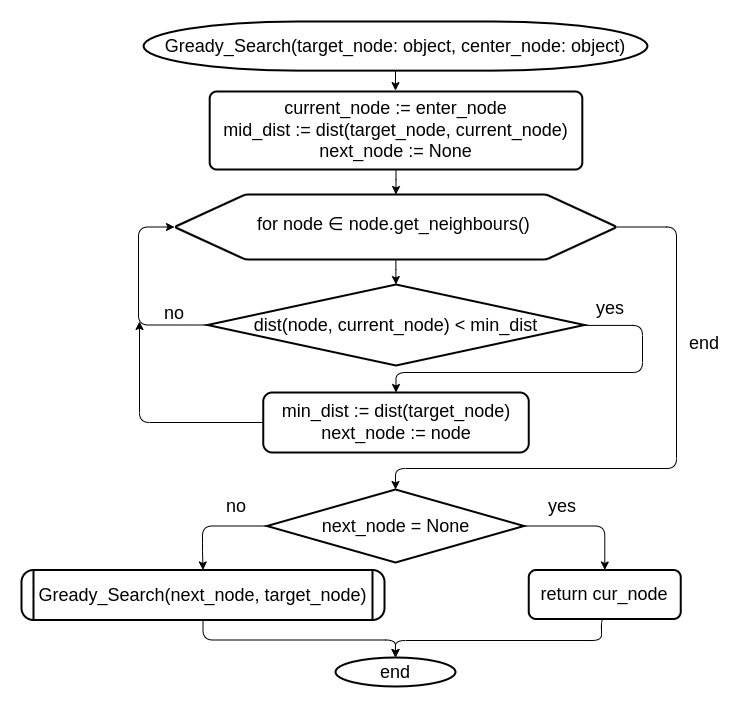
\includegraphics[scale=0.6]{./pictures/Gready_Search.png}
    \caption{Блок схема жадного поиска} \label{grady_search_block_scheme}
\end{figure}

Хочется подметить, что этот алгоритм относится к классу рандомизированных алгоритмов,
так как сам поиск мы начинаем в случайной вершине. На практике такой подход показывает
результат куда лучше, чем если бы стартовая вершина была детерминированной.


Математики из нижнего новгорода, упомянутые выше, предложили способ, как можно улучшить
данный алгоритм, уменьшив вероятность попадания в локальные минимумы. Его блок схему
вы можете найти на рис \ref{multi_search_block_scheme}. Идея заключается в том, чтобы
запустить жадный поиск несколько раз от произвольных вершин и выбрать ту, что окажется ближе.
Данный подход рационален, так как мы подразумеваем, что работаем в "Тесном" графе, а значит,
поиск не будет занимать много времени. Они также пришли к выводу, что достаточно делать
$m \approx \log{n}$ повторений

\begin{figure}[H]
    \centering
    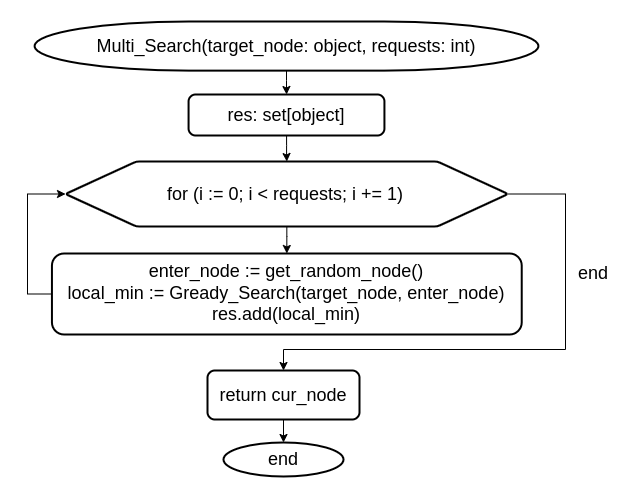
\includegraphics[scale=0.6]{./pictures/Multi_Search.png}
    \caption{Блок схема многократного жадного поиска} \label{multi_search_block_scheme}
\end{figure}

\subsubsection{Построение структуры}

Для построение структуры нам необходимо взять пустой граф и добавлять в него вершины
поэлементно, опираясь на следующий алгоритм: Перед добавлением новой вершины v в граф, 
используя жадный поиск, мы ищем её потенциальное окружение (самые близкие к ней вершины,
присутствующие в графе на данный момент). Выбрав из них только k штук (здесь k - параметр, который
можно варьировать) связываем их с целевой вершиной v. Блок схему данного Алгоритма можно
увидеть на рис \ref{Ponomarenko_graph_block_scheme}.

\begin{figure}[H]
    \centering
    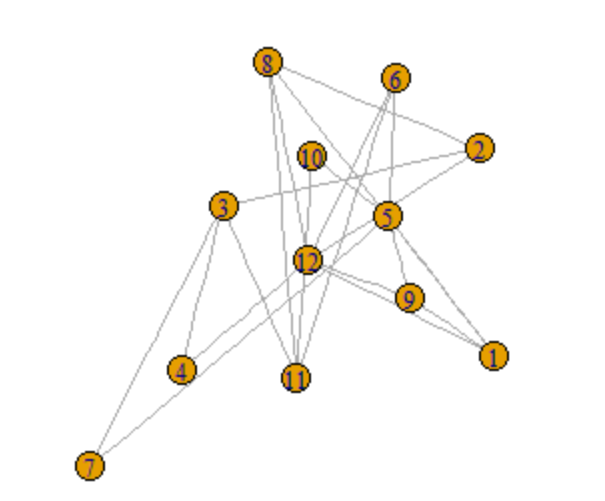
\includegraphics[scale=0.3]{./pictures/random_graph.png}
    \caption{Блок схема многократного жадного поиска} \label{Ponomarenko_graph_block_scheme}
\end{figure}

Хочется подметить несколько важных аспектов:
\begin{itemize}
    \item Граф сильно кластеризован по определению, так как мы связываем вершины только 
    с их ближайшими соседями
    \item Во время создания структуры, данные должны приходить случайно! Игнорирование 
    этого требования может привести к увеличению среднего диаметра
\end{itemize}

Поподробнее остановимся на втором пункте. \\ 
Рассмотрим граф, изображённый на рис \ref{lattice}:

\begin{figure}[H]
    \centering
    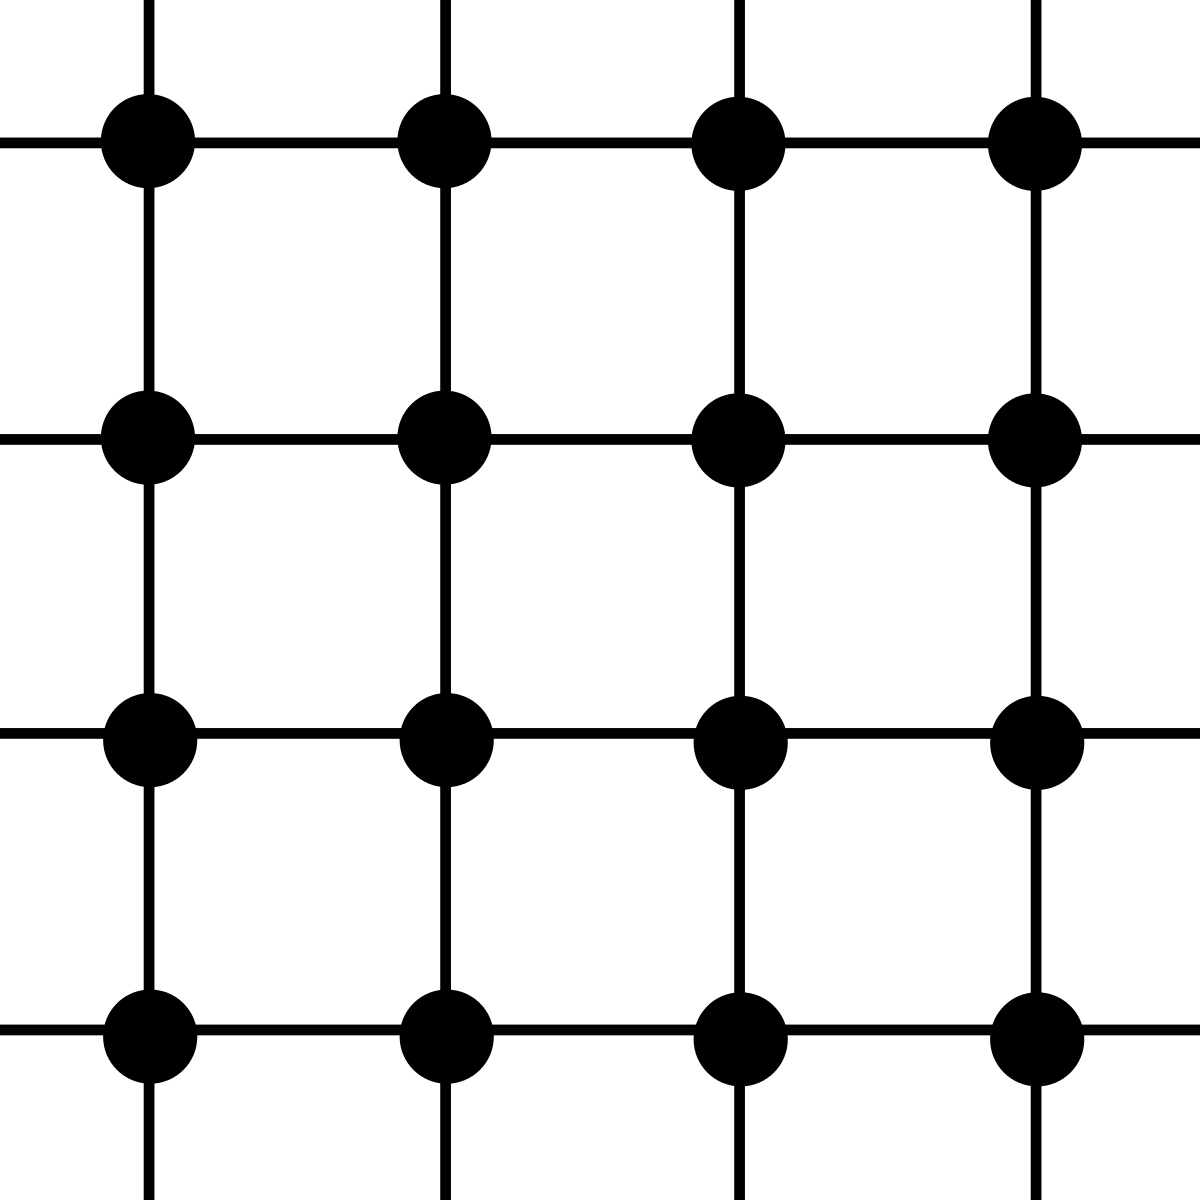
\includegraphics[scale=0.1]{./pictures/Square_grid_graph.svg.png}
    \caption{Пример } \label{lattice}
\end{figure}

Заметим, что даже такой крохотный пример уже имеет средний диаметр $= 2.375$.
Если мы увеличим сетку в 16 раз, то получим средний диаметр $= 9.5$. То есть мы пришли к тому,
что этот граф на 256 вершинах будет иметь средний диаметр больше, чем реальный
граф с 8 млрд вершинами. Но это ещё не всё, заметим, что коэфицент класстеризации тут 
вовсе равен нулю. Так что, этот пример не просто слабо похож на тесный граф, а является 
его полной противоположностью.

Для понимания, как случайность спасает нас в данной ситуации, разделим построение
графа на 2 части:
\begin{itemize}
    \item В самом начале формирование графа, вершин в нём будет немного. Случайный поток данных
    приведёт к тому, что узлы будут достаточно далеко друг от друга (вероятность
    обратного пренебрежимо мала). Поэтому Ближайшие соседи вершины v, которые будут найдены
    посредством жадного алгоритма, будут хоть и самыми близкими из текущих, однако всё
    ещё будут находиться на достаточно большом расстоянии к v. 
    \item С течением времени, ситуация начнёт меняться, ведь вершин будет становиться всё больше,
    а значит, и расположены они будут куда плотнее. Вершины добавленные под конец формирования графа,
    будут иметь соседей, которые будут к ним очень близки не только в сравнении с другими, но и
    по абсолютной величине.
\end{itemize}

Другими словами, в в самом начале формирования графа образуются длинные связи, которые помогают
быстро перемещаться по графу, а ближе к концу - короткие, которые спасают от локальных минимумов.

\subsection{Подход Клайнберга}

    Следующий подход предложил Американский математик Джон Клайнберг. \cite{Kleinberg, Kleinberg2}
%     Следующий подход предложил Американский математик Джон Клайнберг. Перед началом разбора,
% мне бы хотелось сделать некоторую поправку. Джон Клайнберг в своих статьях нигде не 
% упоминает о коэффиценте класстеризации. Вместо этого он говорит только о наличии длинных
% и коротких рёбер. Это немного расширяет класс "Тесных" графов, однако идейно 
% ничего не меняет.

    Изучим заново граф, который изображён на Рис. \ref{lattice}. Он состоит только из
коротких связей, а значит, тесным графом не является. Есть разные способы решить эту проблему,
давайте рассмотрим предложение Джона Клайнберга, так как его метод формирования длинных
рёбер очень естественно вписывается в окружающий нас мир. Идея проста: чем человек дальше от меня, тем меньше
вероятность нашего знакомства. Формально его идею можно записать так, 
Графу даются 2 параметра p, k:
\begin{itemize}
    \item p - радиус. Все вершины, расстояние между которыми меньше или равно p, мы соединяем ребром и 
    и называем короткой связью
    \item k - кол-во длинных связей. После добавления коротких связей, останется только пройтись по всевозможным 
    парам вершин и расставить рёбра в зависимости от следующего распределения:
\end{itemize}

\begin{equation} \label{edges_distribution}
    P(u \rightarrow v) = \frac{1}{d(u, v)^r}\frac{1}{C}, \text{ где } C = \sum_{u \neq z \in V}\frac{1}{d(u, z)^r}
\end{equation}

Во время своего исследования, он пришёл к выводу, что наилучший результат достигается при 
r = d, где d - размерность пространства. Причём кол-во длинных рёбер должно быть 
примерно равно $q = \log{n}$.

\subsubsection{Построение структуры}
Алгоритм построения представлен в виде блок схемы. Хочу заметить, что асимптотическая
сложность построения данной стркутуры очень большая ($O(n^2)$), что делает её мало где применимым.
Однако граф Клайнберга - является больше идеей. Её можно внедрять в другие структуры для 
их модификации 

\begin{figure}[H]
    \centering
    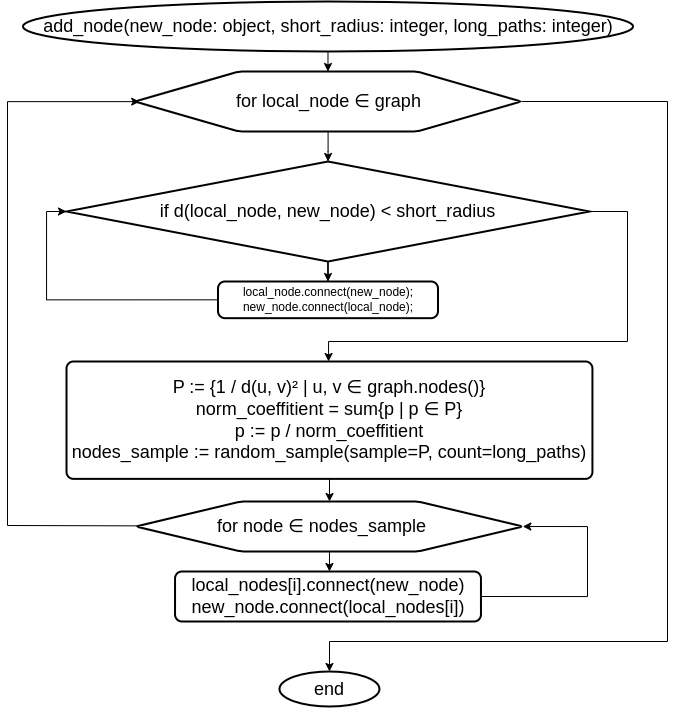
\includegraphics[scale=0.6]{./pictures/Kleinberg_add_node.png}
    \caption{Блок схема построение графа по методу Джона Клайнберга} \label{Kleinberg_graph_block_scheme}
\end{figure}





\subsection{Предложени по модификации}

Оба подхода хорошо себя показывают в проблеме поиска ближайшего соседа. Однако Хочется
предложить модификацию того алгоритма, который был предложен Нижегородскими математиками.

Есть гипотеза, что кол-во длинных рёбер, которые образовываются посредством данного алгоритма
недостаточно для эффективной навигации по графу. Кроме того, нужно следить за тем, чтобы данные
шли случайно, что тоже иногда может быть не очень удобно.

Для решения этой проблемы, предлагаю объединить данный подход с классическим методом построения
тесного графа Уоттса–Строгаца. Идея заключается в следующем:

\begin{itemize}
    \item [1)] Жадным поиском ищем окружение вершины v, которую хотим добавить
    \item [2)] Выбираем k(параметр) ближайших вершин.
    \item [3)] Связываем вершину v лишь с некоторыми из выбранных вершин. Вероятность ребра 
    теперь будет являться отдельным параметром и задаваться заранее
    \item [4)] Каждое непроведённое ребро будет компенсироваться другим. Это новое ребро будет связывать
    нашу вершину v с другой абсолютно случайно выбранной вершиной в графе.
\end{itemize}

В практической части, я собираюсь проверить эффективность данного подхода в сравнении с другими методами.
А также подобрать параметр p, при котром модель будет давать наилучшие результаты.
\section{Практическая часть}

\subsection{Описание абстракций}

Для начала, я бы хотел описать, какие классы были реализованы, 
каким образом и для чего они преднозначены.

\subsubsection{Класс Graph}

Данный граф является основным. Он реализует все самые необходимые инструменты для
взаиможействия с графами, такие как: добавление вершины в граф, добавление ребра, очистка графа
и т.д. 

Данная абстракция была реализована на основе хэш таблицы (std::unordered\_map). 
Такой контейнер был выбран не случайно, так как он осуществляет очень быстрый доступ 
к произвольным данным (Добавление, поиск, удаление за O(1)).

Этот класс является шаблонным и может хранить в себе объекты любой природы. Главное, чтобы
они удовлетворяли двум требованиям:

\begin{itemize}
    \item Наличие перегрузки оператора равенства 
    \item Наличие функции хэширования (для std::unordered\_map)
\end{itemize}
Объявление класса: 

\begin{verbatim}
    template<typename TObject, typename HashFunc>
    class Graph {
        std::unordered_map<TObject, std::vector<TObject>, HashFunc> graph;
        std::vector<TObject> nodes;
        size_t size;
    public:
        Graph() = default;
        Graph(const Graph& g) = delete;
        Graph(Graph&& g) = delete;

        void add_node(const TObject& p);
        void add_edge(const TObject& p1, const TObject& p2);
        void delete_edge(const TObject& p1, const TObject& p2);
        void clear();
        std::size_t get_size() const;
        bool consists_node(const TObject& p) const;
        bool consists_edge(const TObject& p1, const TObject& p2) const;
        const std::vector<TObject>& get_neighbours(const TObject& p) const;
        const TObject& get_random_node() const;
        friend std::ostream& operator<< <>(std::ostream& out, 
                                           const Graph& graph);
        ~Graph() = default;
    };
\end{verbatim}
Хочу отдельное внимание обратить на метод get\_random\_node. Его необходимость 
станет очевидна вдальнейшем, пока мне бы хотелось рассказать о дилеме, с которой я столкнулся
во время её написания. Для реализации этого метода, мы должны иметь возможность выбирать из хэш таблицы
любой ключ случайно, однако это возможно сделать только за линейное время, из-за отсутствия в 
unordered\_map обращения по индексу. Для решения этой проблемы мною было принято решение создать отдельный
вектор из объектов, так как в нём, используя случайные индексы, мы без проблем сможем выбрать 
абсолютно любой объект за O(1). 
Это привело к следующим последствиям:
\begin{itemize}
    \item Увеличение кол-во памяти необходимое для хранения структуры
    \item Ухудшение асимптотической скорости удаление выбранных элементов (до линейной)
\end{itemize}
Однако все эти недостатки никак негативно не повлияли конкретно в решении задач текущего проекта 


\subsubsection{Классы Point и Point3D}

Данные абстракции в моём проекте используются, как объекты, вершины графа. 
Они являются больше примером для наглядной демонстрации работы других классов.
Заго\-ловки выглядят следующим образом:


\begin{verbatim}
    class Point {
        public:
            double x;
            double y;
            Point() = default;
            Point(const Point& p) = default;
            Point(Point&& p) = default;
            Point(double x, double y);
            friend std::ostream& operator<<(std::ostream& out, 
                                            const Point& p);
            bool operator==(const Point& p) const;
            static double dist(const Point& p1, const Point& p2);
            class HashPoint {
            public:
                std::size_t operator()(const Point& p) const;
            };
            ~Point() = default;
        };
        class Point3D {
        public:
            double x;
            double y;
            double z;
            Point3D() = default;
            Point3D(const Point3D& p) = default;
            Point3D(Point3D&& p) = default;
            Point3D(double x, double y, double z);
            friend std::ostream& operator<<(std::ostream& out, 
                                            const Point3D p);
            bool operator==(const Point3D p) const;
            static double dist(const Point3D p1, const Point3D p2);
            class HashPoint {
            public:
                std::size_t operator()(const Point3D& p) const;
            };
        };
\end{verbatim}

\subsubsection{Класс Nswg} 


Данный класс является абстрактным. Внутри он содержит всё необходимое для реали\-зации
жадного поиска, однако на этом всё. Процесс формирования самого графа ложится на плечи
потомков (поэтому метод load\_nodes помечен, как виртуальный). Данное ре\-шение было принято, чтобы не копировать в каждый новый класс одинаковые 
методы жадного поиска.

\begin{verbatim}
    template<typename TObject, typename HashFunc>
    class Nswg {
    protected:
        Graph<TObject, HashFunc> graph;
        std::size_t sum_of_degrees = 0;

        class ClosestToCompare {
            const TObject& base;
        public:
            ClosestToCompare(const TObject& base) : base(base) {};
            bool operator()(const TObject& p1, const TObject& p2) const;
        };

        void multi_search(const TObject& target_node, 
                          std::set<TObject, ClosestToCompare>& res, 
                          std::size_t count) const;

    public:
        virtual void load_nodes(const std::vector<TObject>& objects) = 0;
        double get_mean_deg() const;
        double get_cc() const;

        const std::vector<TObject>& get_nodes() const;

        ~Graph() = default;
        const TObject& greedy_search(const TObject& target_node, 
                                     const TObject& start_node) const;
        std::pair<TObject, double> get_best_element(const TObject& target, 
                                                    std::size_t count) const;

        const std::vector<TObject>& get_neighbours(const TObject& p) const;
        const TObject& get_random_node() const;
        void clear();
        std::size_t get_size() const;
    };
\end{verbatim}

Также, хотелось бы ещё рассказать почему я использую внутренние дополнительный класс ClosestToCompare(). 
Как я уже описывал, в жадном поиске нам нужно искать k вершин наиболее близких с нашей.
Постоянные сортировки могли достаточно сильно ухудшить производительность модели, поэтому я принял решение, 
написать предикат, который будет сортировать вершины в set() сразу так, как нужно:
\begin{itemize}
    \item В конструктор класса мы передаём объект v
    \item Чем ближе вершина к v, тем первее она будет находится в set.
    \item Однако возникнет проблема, что 2 узла на одном расстоянии теперь будут считаться
    одинаковыми, а значит, в set добавится только один из них. Для решения этой проблемы, мне пришлось
    добавить второе условие, котороые сравнивает хеши вер\-шин и сортирует на основе их значений:
\end{itemize}

\begin{verbatim}
    template<typename TObject, typename HashFunc>
    bool Nswg<TObject, HashFunc>::ClosestToCompare::operator()(
                                                    const TObject& p1, 
                                                    const TObject& p2) const {
        double d1 = TObject::dist(p1, base);
        double d2 = TObject::dist(p2, base);
        if (d1 != d2) {
            return TObject::dist(p1, base) < TObject::dist(p2, base);
        } else {
            HashFunc hash;
            return hash(p1) < hash(p2);
        }
    }
\end{verbatim}

\subsubsection{NNGraph}

Является наследником класса Nswg и с помощью метода load\_nodes реализует постро\-ение графа.
Испрользует подход математиков из Нижнего Новгорода, упомянутых выше
Алго\-ритм построения уже был разобран в блок схеме выше.

\begin{verbatim}
    template<typename TObject, typename HashFunc>
    class NNGraph : public Nswg<TObject, HashFunc> {
        std::size_t queries_count = 5;
        std::size_t edges_count = 7;
    public:
        NNGraph(std::size_t queries_count = 5, std::size_t edges_count = 7);
        // NNGraph(const std::vector<TObject>& objects);

        NNGraph(const NNGraph& pg) = delete;
        NNGraph(NNGraph&& pg) = delete;

        void add_node(const TObject& obj);
        void load_nodes(const std::vector<TObject>& objects) override;

        friend std::ostream& operator<< <>(
                             std::ostream& out, 
                             sconst NNGraph<TObject, HashFunc>& pgraph);

        ~NNGraph() = default;
    };
\end{verbatim}


\subsubsection{KleinbergGraph}

Является наследником класса Nswg и с помощью метода load\_nodes реализует постро\-ение графа.
Алгоритм построения уже был разобран в блок схеме выше.

\subsubsection{RandomGraph}

Данный класс был реализован на основе графов Erdos-Renye. Был создан для срав\-нительного анализа

\begin{verbatim}
    template<typename TObject, typename HashFunc>
    class RandomGraph : public Nswg<TObject, HashFunc> {
        double mean_neighbours;
    public:
        RandomGraph(double mean_neighbours);
        RandomGraph(const RandomGraph& rg) = delete;
        RandomGraph(RandomGraph&& rg) = delete;

        void load_nodes(const std::vector<TObject>& objects) override;

        ~RandomGraph() = default;
    };
\end{verbatim}

\subsubsection{Figure}

Данная абстракция была создана с целью упрощения визуализации графов и гра\-фиков.
Он работает по очень простому принципу: Под капотом она пишет скрипт на питоне, который
записывает в отдельный файл. После чего в отдельном процессе этот файл запускается и 
выводит данные в виде графиков. В Питоне я использовал библиотеку Plotly


\begin{verbatim}
    class Figure {
        std::ofstream script;
        std::string name;
        void write_vector_as_list(const std::string& name, 
                                  const std::vector<double> &data);
    public:
        Figure() = delete; // TODO: why not
        Figure(const std::string& name);
        Figure(const Figure& f) = delete;
        Figure(Figure&& f) = delete;
        void add_graph(const Nswg<Point, Point::HashPoint>& g,
                       std::size_t marker_size,
                       std::size_t line_width,
                       const std::string& marker_color,
                       const std::string& line_color,
                       const std::string& name);
        void update_title(const std::string& title);
        void add_markers_and_lines(const std::vector<double>& x,
                                   const std::vector<double>& y,
                                   std::size_t marker_size,
                                   std::size_t line_width,
                                   const std::string& marker_color,
                                   const std::string& line_color,
                                   const std::string& name);
        void add_markers(const std::vector<double>& x,
                         const std::vector<double>& y,
                         std::size_t marker_size,
                         const std::string& marker_color,
                         const std::string& name);
        void add_line(const std::vector<double>& x,
                      const std::vector<double>& y,
                      std::size_t line_width,
                      const std::string& line_color,
                      const std::string& name);
        void update_xaxes(const std::string& x_title, 
                          const std::string& axis_type);
        void update_yaxes(const std::string& y_title, 
                          const std::string& axis_type);
        void show();
        ~Figure();
    };
\end{verbatim}





\section{Заключение}

В заключение хочется сказать, что все необходимы задачи были выполнены:
\begin{itemize}
    \item Были изучены разные виды графовых структур для поиска ближайшего соседа, а 
    также 
    \item Были расписаны их преимущества и недостатки
    \item Был полностью изучен феномен тесного мира
    \item Были изучены 2 структуры, которые опираются на этот метод
    \item Были разработаны очень удобные абстракции для работы с графовыми структурами
    \item Был проведён сравнительный анализ структур
\end{itemize}

Обе эти структуры показали свою эффективность в сравнении со случайным графом, за короткое 
кол-во путей они давали результат с очень малой ошибкой, что показывает их эффективность
и применимость. Однако хочется сделать небольшую пометку, построение графа Клайнберга занимает очень
много времени($O(n^2)$) Поэтому его алгоритм лучше использовать, как идею для внедрения в другие типы графов. 
Под идеей имеется в виду расстановка рёбер, опираясь на распределение. Алгоритм построения графа,
который изучали Нижегородские математики, работает достаточно эффективно как по времени, так и по памяти,
поэтому он применим в чистом виде. 

Реализованные структуры очень легко масштабируются, можно внедрить ещё огромное кол-во других абстракций, которые
без "костылей" впишутся в общую структуру классов. Поэтому данный проект можно продолжать развивать,
я планирую сделать свою библиотеку для работы с разными графовыми структурами. Возможно, со
специальными абстракциями для тестирования.

\printbibliography

\end{document}
